\documentclass[submit]{harvardml}



% You don't need to change these.
\course{CS181-S18}
\assignment{Assignment \#2 v1.1}
\duedate{11:59pm Feb 23rd, 2018}

\usepackage[OT1]{fontenc}
\usepackage[colorlinks,citecolor=blue,urlcolor=blue]{hyperref}
\usepackage[pdftex]{graphicx}
\usepackage{subfig}
\usepackage{fullpage}
\usepackage{amsmath}
\usepackage{amssymb}
\usepackage{color}
\usepackage{soul}
\usepackage{todonotes}
\usepackage{listings}
\usepackage{common}
\usepackage{bm}

\usepackage[mmddyyyy,hhmmss]{datetime}

\definecolor{verbgray}{gray}{0.9}

\lstnewenvironment{csv}{%
  \lstset{backgroundcolor=\color{verbgray},
  frame=single,
  framerule=0pt,
  basicstyle=\ttfamily,
  columns=fullflexible}}{}

\begin{document}


%%% Change the assignment details here:
{
  \begin{center}
{\Large Homework 2: Bayesian Methods and Multiclass Classification}\\
\end{center}
}
\subsection*{Introduction}

This homework is about Bayesian methods 
and  multiclass classification. In lecture we have
primarily focused on binary classifiers trained to discriminate
between two classes. In multiclass classification, we discriminate
between three or more classes. We encourage you to first read the
Bishop textbook coverage of these topic, particularly: Section 4.2
(Probabilistic Generative Models), Section 4.3 (Probabilistic
Discriminative Models).
%, and, if MLE is troublesome, review 
%the materal Section 1
%and lecture 3.

As usual, we imagine that we have the input matrix $\boldX \in
\reals^{n \times m}$ (or perhaps they have been mapped to some basis
$\bm{\Phi}$, without loss of generality) but our outputs are now
``one-hot coded''.  What that means is that, if there are~$c$ output
classes, then rather than representing the output label $y$ as an
integer~${1,2,\ldots,c}$, we represent $\boldy$ as a binary vector of
length~$c$. These vectors are zero in each
component except for the one corresponding to the correct label, and
that entry has a one.  So, if there are 7 classes and a particular
datum has label 3, then the target vector would be~${C_3 = [0,0,1,0,0,0,0]}$. 
If there are $c$ classes, the set of possible outputs is $\{C_1 \ldots C_c \} = \{C_k\}_{k=1}^c$.
Throughout the assignment we will assume
that output $\boldy \in \{C_k\}_{k=1}^c$.\\

The problem set has three problems: 
\begin{itemize}
\item In the first problem, you will explore the properties of Bayesian
estimation methods for the Bernoulli model as well as the special
case of Bayesian linear regression with a simple prior.
%
\item  In the second
problem, you will dive into  matrix algebra and the methods behind
generative multiclass classifications. You will extend the discrete classifiers  
that we see in  lecture to a Gaussian model.
%
\item Finally, in the third problem, you will implement 
 logistic regression as well as a generative classifier 
from close to scratch.
%
\end{itemize}

\newpage
\begin{problem}[Bayesian Methods, 10 pts]

  This question helps to build your understanding of the
  maximum-likelihood estimation (MLE) vs. maximum a posterior estimator
  (MAP) and posterior predictive estimator, first in the
  Beta-Bernoulli model and then in the linear regression setting.\\

First consider the Beta-Bernoulli model (and see lecture 5.) 
%
\begin{enumerate}
\item[1.] Write down the expressions for the MLE, MAP and posterior predictive
distributions, and for
a prior $\theta\sim Beta(4,2)$ on the
parameter of the Bernoulli,
and  with data $D= 0, 0, 1, 1, 0, 0, 0, 0, 1, 0, 1, 1,$ 
$1, 0, 1, 0$, plot 
the three different
estimates after each additional
sample.
%
\item[2.] Plot the posterior distribution (prior for 0 examples) on $\theta$ after 0, 4, 8, 12 and 16
examples. (Using whatever tools you like.)
%
\item[3.] Interpret the differences you see between the three different
estimators.
%
%note, initial skew is to large 1, but data has $\theta=0.4$
%
\end{enumerate}

Second, consider the Bayesian Linear Regression model, with
data $D=\{(\boldx_i,y_i)\}_{i=1}^n$, $\boldx_i\in\mathbb{R}^m$,
 $y_i\in\mathbb{R}$, and generative model 
%
$$
y_i\sim\mcN(\boldw^\top\boldx_i,\beta^{-1})
$$
for (known) precision $\beta$ (which is just the reciprocal
of the variance). Given this, the likelihood of the
data is $p(\boldy|\boldX,\boldw) = \mcN(\boldy|\boldX\boldw,\beta^{-1}\mathbf{I})$. Consider the special case of 
an isotropic (spherical) prior on weights, with
%
$$
p(\boldw)=\mcN(\boldw|\bold0,\alpha^{-1}\boldI)
$$

This prior makes sense when you have little prior information and do not know much about the relationship among features so you can simplify by assuming independence.

\begin{enumerate}

\item[4.] Using the method in lecture of taking logs, expanding and pushing terms
that don't depend on $\boldw$ into a constant, and finally collecting
terms and completing the square, confirm that the posterior on
weights after data $D$ is $\boldw\sim\mcN(\boldw|\boldm_n,\boldS_n)$,
where
%
\begin{align*}
\boldS_n&=(\alpha\boldI+\beta\boldX^\top\boldX)^{-1}\\
\boldm_n&=\beta\boldS_n\boldX^\top\boldy
\end{align*}
\end{enumerate}
\end{problem}

%\subsection*{2. Mooooar matrix calculus [10 pts]}
%%%%%%%%%%%%%%%%%%%%%%%%%%%%%%%%%%%%%%%%%%%%%
% Problem 2
%%%%%%%%%%%%%%%%%%%%%%%%%%%%%%%%%%%%%%%%%%%%%
\begin{problem}[Return of matrix calculus, 10pts]

  Consider now a generative $c$-class model.  We adopt class prior
  $p(\boldy = C_k; \bpi) = \pi_k$ for all $k \in \{1, \ldots, c\}$
(where $\pi_k$ is a parameter of the prior).
%
%that define the prior. 
Let  $p(\boldx|\boldy=C_k)$ denote
the class-conditional density of features $\boldx$ (in this
case for class $C_k$). Consider the data set $D = \{(\boldx_i,
\boldy_i)\}_{i=1}^n$ where as above $\boldy_i \in \{C_k\}_{k=1}^c$ is
encoded as a one-hot target vector. 
%
\begin{enumerate}
  \item Write out the negated log-likelihood of the data set,
    $-\ln p(D ; \bpi)$.
%
  \item Since the prior forms a distribution, it has the constraint that
    $\sum_k\pi_k - 1 = 0$.  Using the hint on
Lagrange multipliers below, give the
    expression for the maximum-likelihood estimator for the prior
    class-membership probabilities, i.e.
    $\hat \pi_k.$
    Make sure to write out the intermediary equation you need
    to solve to obtain this estimator. Double-check your answer: the final
    result should be very intuitive!
\end{enumerate}

    For the remaining questions, let the 
    class-conditional probabilities be Gaussian distributions with 
the same covariance matrix
    $$p(\boldx | \boldy = C_k) = \mathcal{N}(\boldx |  \bmu_k, \bSigma), \text{\ for\ }k \in \{1,\ldots, c\}$$
%
and different means $\bmu_k$ for each class.
%
    \begin{enumerate}
  \item[3.] Derive the gradient of the negative log-likelihood with respect to vector $\bmu_k$.
    Write the expression in matrix form as a function of the variables defined
    throughout this exercise. Simplify as much as possible for full credit.
  \item[4.] Derive the maximum-likelihood estimator for vector $\bmu_k$. Once
    again, your final answer should seem intuitive.
  \item[5.] Derive the gradient for the negative log-likelihood with respect to the
    covariance matrix $\bSigma$ (i.e., looking
to find an MLE for the covariance). 
Since you are differentiating with respect to a
    \emph{matrix}, the resulting expression should be a matrix!
%
  \item[6.] Derive the maximum likelihood estimator of the covariance matrix.
\end{enumerate}

\paragraph{Hint: Lagrange Multipliers.} Lagrange Multipliers are a method for
optimizing a function $f$ with respect to an
equality constraint, i.e. 
\[\min_{\boldx} f(\boldx)\ \text{s.t.}\ g(\boldx) = 0.\]

This can be turned into an unconstrained problem by introducing a
Lagrange multiplier $\lambda$ and constructing the Lagrangian function,
\[L(\boldx, \lambda) =  f(\boldx) + \lambda g(\boldx).\]

It can be shown that it is a necessary condition that the optimum 
is a critical point of this new function. We can find this point by solving two equations:

\[\frac{\partial L(\boldx, \lambda)}{\partial  \boldx} = 0  \ \ \text{and}\  \  \frac{\partial L(\boldx, \lambda)}{\partial \lambda} = 0 \]


\paragraph{Cookbook formulas.} Here are some formulas you might want to consider
using to compute difficult gradients. You can use them  in the homework
without proof. If you are looking to hone your matrix calculus skills, try to
find different ways to prove these formulas yourself (will not be part of the
evaluation of this homework). In general, you can use any formula from the matrix cookbook,
as long as you cite it. We opt for the following common notation:
$\boldX^{-\top} := (\boldX^{\top})^{-1}$
\begin{align*}
  & \frac{\partial \bolda^\top \boldX^{-1} \boldb}{\partial \boldX} = - \boldX^{-\top} \bolda \boldb^\top \boldX^{-\top} \\
  & \frac{\partial \ln | \det (\boldX) |}{\partial \boldX} = \boldX^{-\top}
 \end{align*}
 \end{problem}





\newpage

\subsection*{3. Classifying Fruit [15pts]}
You're tasked with  classifying three different kinds of fruit, based on their
heights and widths.  Figure~\ref{fig:fruit} is a plot of the data.  Iain Murray
collected these data and you can read more about this on his website at
\url{http://homepages.inf.ed.ac.uk/imurray2/teaching/oranges_and_lemons/}.  We
have made a slightly simplified (collapsing the subcategories together) version
of this available as \verb|fruit.csv|, which you will find in the Github repository.
The file has three columns: type (1=apple, 2=orange, 3=lemon), width,
and height.  The first few lines look like this:
\begin{csv}
fruit,width,height
1,8.4,7.3
1,8,6.8
1,7.4,7.2
1,7.1,7.8
...
\end{csv}
\begin{figure}[h]
\centering
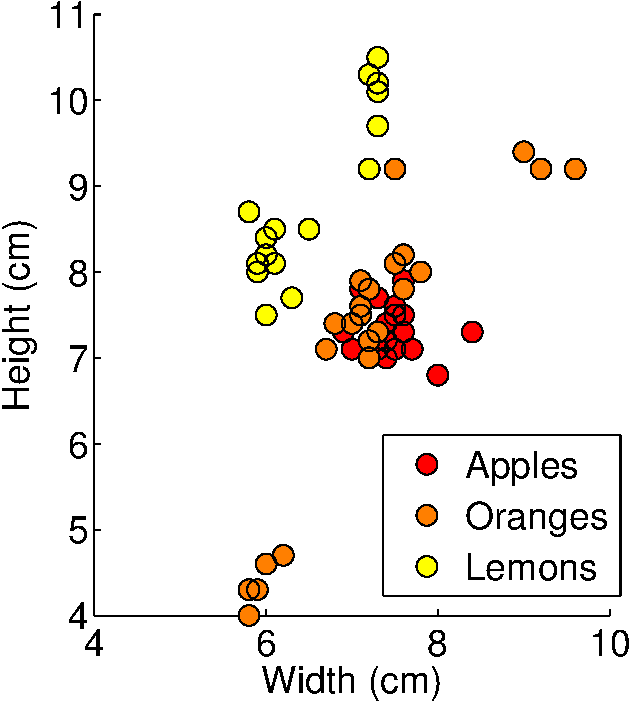
\includegraphics[width=0.5\textwidth]{fruit}
\caption{Heights and widths of apples, oranges, and lemons.  These fruit were
purchased and measured by Iain Murray:
\url{http://homepages.inf.ed.ac.uk/imurray2/teaching/oranges_and_lemons/}.}
\label{fig:fruit}
\end{figure}
\begin{problem}[Classifying Fruit, 15pts]
  You should implement the following:
\begin{itemize}
\item The three-class generalization of logistic regression, also
  known as softmax regression, for these data. You will do this by implementing
  gradient descent on the negative log likelihood. You will need to find good values for the learning rate $\eta$ and regularization strength $\lambda$. See the third practice problem in the section 3 notes for information about multi-class logistic regression, softmax, and negative log likelihood.
%
\item A generative classifier with Gaussian
  class-conditional densities, as in Problem~3. In particular, make
  two implementations of this, one with a shared covariance matrix
  across all of the classes, and one with a separate covariance being
  learned for each class.  Note that the staff implementation can
  switch between these two by the addition of just a few lines of
  code. In the separate covariance matrix case, the MLE for the
  covariance matrix of each class is simply the covariance of the data
  points assigned to that class, without combining them as in the
  shared case.
\end{itemize}
You may use anything in  \texttt{numpy} or \texttt{scipy}, except for \texttt{scipy.optimize}. That being said, if you happen to find a function in \texttt{numpy} or \texttt{scipy} that seems like it is doing too much for you, run it by a staff member on Piazza. In general, linear algebra and random variable functions are fine. The controller file is \texttt{problem3.py}, in which you will specify hyperparameters. The actual implementations you will write will be in \texttt{LogisticRegression.py} and \texttt{GaussianGenerativeModel.py}.


You will be given class interfaces for \texttt{GaussianGenerativeModel} and \texttt{LogisticRegression} in the distribution code, 
and the code will indicate certain lines that you should not change in your final submission. Naturally, don't change these.
These classes will allow the final submissions to have consistency. There will also be a few hyperparameters that are set to
irrelevant values at the moment. You may need to modify these to get your methods to work.
The classes you implement follow the same pattern as scikit-learn, so they should be familiar to you. The distribution code currently outputs nonsense predictions just to show what the high-level interface should be, so you should completely remove the given \texttt{predict()} implementations and replace them with your implementations.

\begin{itemize}
\item The \texttt{visualize()} method for each classifier will save a plot that will show the decision boundaries. You should include these in this assignment.
\item Which classifiers model the distributions well?
\item What explains the differences?

\end{itemize}

In addition to comparing the decision boundaries of the three models visually:
\begin{itemize}

\item For logistic regression, plot negative log-likelihood loss with iterations on the x-axis and loss on the y-axis for several configurations of hyperparameters. Note which configuration yields the best final loss. Why are your final choices of learning rate ($\eta$) and regularization strength ($\lambda$) reasonable? How does altering these hyperparameters affect convergence? Focus both on the ability to converge and the rate at which it converges (a qualitative description is sufficient).

\item For both Gaussian generative models, report negative log likelihood. In the separate covariance matrix case, be sure to use the covariance matrix that matches the true class of each data point.

\end{itemize}

Finally, consider a fruit with width 4cm and height 11cm.  To what
class do each of the classifiers assign this fruit? What do these results tell you about the classifiers' ability to generalize to new data?  Repeat
for a fruit of width 8.5cm and height 7cm.

\end{problem}

\newpage
\subsection*{Calibration [1pt]}
Approximately how long did this homework take you to complete?

\subsection*{Name, Email, and Collaborators}

Name:

Email:

Collaborators:


\end{document}
